\documentclass[10pt,twocolumn,letterpaper]{article}
\usepackage[margin=0.72in,columnsep=0.26in]{geometry}
\usepackage[T1]{fontenc}
\usepackage{times}
\usepackage{microtype}
\usepackage{amsmath,amssymb,amsthm}
\usepackage{graphicx}
\graphicspath{{../figures/out/}}
\usepackage{booktabs}
\usepackage{xcolor}
\usepackage[numbers,sort&compress]{natbib}
\usepackage[colorlinks=true,linkcolor=blue!50!black,citecolor=blue!50!black,urlcolor=blue!50!black]{hyperref}
\hypersetup{pdftitle={Three Objects, One Image: Depth Networks Read an Impossible Figure One Joint at a Time},
  pdfauthor={Itamar Shalom, Yalli Lavi, Dotan Greenspan, Shalom Biton}}
\usepackage[font=small,labelfont=bf]{caption}
\setlength{\abovecaptionskip}{3pt}
\setlength{\belowcaptionskip}{-3pt}
\setlength{\textfloatsep}{8pt plus 2pt minus 2pt}
\setlength{\floatsep}{6pt plus 2pt minus 2pt}
\setlength{\bibsep}{0pt plus 0.3ex}
\newtheorem{proposition}{Proposition}
\newtheorem{corollary}{Corollary}
\newcommand{\doi}[1]{doi:~\href{https://doi.org/#1}{\nolinkurl{#1}}}
\renewcommand{\bibfont}{\raggedright}

\title{\vspace{-0.55in}Three Objects, One Image:\\Depth Networks Read an Impossible Figure One Joint at a Time}
\author{Itamar Shalom \quad Yalli Lavi \quad Dotan Greenspan \quad Shalom Biton\\
{\small Modern Computer Vision, Technion \quad\textbullet\quad Code: \url{https://github.com/Itamarshalom/three-objects-one-image}}}
\date{\vspace{-0.3in}}

\begin{document}
\maketitle

\begin{abstract}
A Penrose-triangle drawing is, pixel for pixel, the orthographic image of three straight-bar objects, each an open
chain with its gap at a different joint, so these three readings and their depth are known exactly. Around the loop
every bar comes nearer, so a depth map with rigid bars must jump back somewhere. For an ideal predictor that believes in the
three objects, the loss decides where. A squared error splits the jump among the joints and an absolute error puts it at
a majority object's gap; either way the joints pay the whole mismatch. We test ten frozen depth networks
(Depth Anything V2, MiDaS, ZoeDepth, Lotus, Marigold). All of them find the gap when it is
visible. On the impossible image their joints pay between $-0.19$ and $0.32$ of the mismatch: each joint gets about the
step it gets as an ordinary joint (within 5--15\% of the jump), and the mismatch is left in the bars. Revealing 64 to 688
pixels of the real gap restores half of the jump, and multi-step diffusion samples do not commit to an object either.
The networks behave as if they read each junction locally and never check the loop.
\end{abstract}

\section{Introduction}
Depth from a single image is ill-posed, so a trained network returns a statistic of the scenes it considers
consistent with its input, and its loss decides which: the posterior mean under a squared error, the per-pixel median
under an absolute error, a sample for a diffusion model. When the plausible scenes form a few distinct modes these
statistics differ sharply. Natural images do not reveal the set of correct answers, so which statistic a network
actually returns has been hard to measure.

We build images for which the set is known. An open chain of three straight bars, seen from one special direction,
closes into the Penrose triangle~\cite{penrose1958impossible}. Placing the gap at any of the three corners gives the same
picture, so under a prior of three rigid right-angled bars (other polyhedra can also produce it~\cite{sugihara2000impossible})
the image has exactly three upright readings, and we render all three with their exact depth (Fig.~\ref{fig:hero}). No depth map can keep every bar rigid and still close the loop: it
must jump back by a fixed total $T$ somewhere, Penrose's cohomology obstruction~\cite{penrose1992cohomology}. A valid
object pays $T$ with one jump at its gap; the average of the three pays $T/3$ at every joint.

Our contribution is such a test image with the exact depth of its readings, the answers the common training losses
give for it (Sec.~\ref{sec:theory}), and a scale-free read-out that places ten networks against them. On the impossible
image the networks read each joint as an ordinary joint and leave the loop's mismatch in the bars. In the terms of classical line-drawing analysis, impossible figures are
drawings whose junctions are consistent one by one but not together~\cite{huffman1971impossible,clowes1971seeing}; the
networks behave like a junction labeller that never makes the global check.

\paragraph{Related work.}
Jiang et al.~\cite{jiang2019illusions} asked whether a depth network reads impossible figures locally or globally;
anecdotes (``a conveniently-sized gap'') suggested global structure, and they left measuring it to future work. CNNs
fail to tell possible from impossible objects~\cite{heinke2021failure}. Han et al.~\cite{han2024multistable}
found that depth networks commit to one of two readings
of shading images; our ambiguity is geometric and lets us compare losses on a shared backbone. Benchmarks probe depth
networks with illusions, where the flat surface is correct~\cite{yao2025illusion,nguyen2026mirage}, and with
transparent scenes, where two layers are valid~\cite{xu2026onescene}. The view that regression
averages the explanations of an ill-posed input~\cite{blau2018perception} motivates iterative
restoration~\cite{delbracio2023indi}; we test it where they are enumerable.

\begin{figure*}[t]
\centering
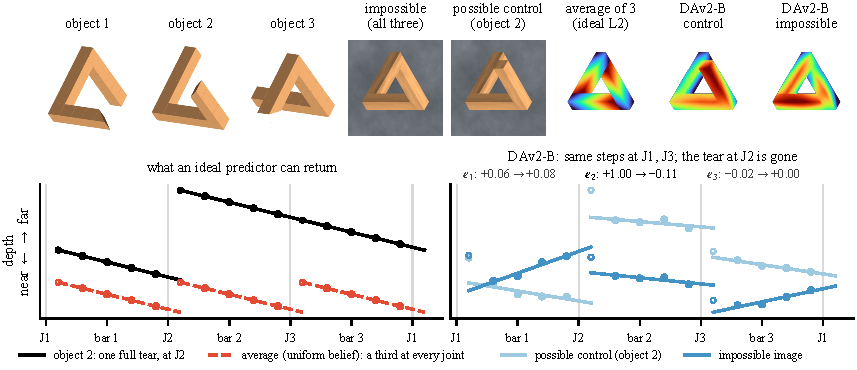
\includegraphics[width=\textwidth]{fig_hero.pdf}
\caption{\textbf{Three objects, one image, one joint at a time.} Top: three straight-bar objects ($12^\circ$ off the
special view) give one impossible image; the control shows object 2's gap; depth of the objects' average and of Depth
Anything V2-B (red = near; layout $90^\circ$). Bottom: loop profiles (dots: cube depths, hollow corner cubes unused;
lines: bar fits; the average is shifted down for display). Right: on the impossible image J2 gets an ordinary step while J1 and J3 keep theirs (excess tear $e_j$, control $\to$ impossible, Sec.~\ref{sec:readout}: 1 = the control's tear, 0 = an ordinary step).}
\label{fig:hero}
\end{figure*}

\section{Method}
\subsection{Three objects with one image}
The loop is built from unit cubes: $n{-}1$ steps along $+x$, $+y$ and $+z$ ($n=6$, 15 cubes). Viewed orthographically
along $v=(1,1,1)/\sqrt3$ the chain's end projects onto its start. Object $k$ starts the chain at corner $k$ (cube $c_k$), which
moves the cubes before it by $(n{-}1)(1,1,1)$, a translation along $v$ that leaves their image unchanged. So every
cube has the same footprint in all three objects and $d_k=d_1-T\,\mathbf 1[c<c_k]$ with $c$ the cube index and
$T=(n{-}1)\sqrt3$. At its gap, the end of object $k$'s nearer bar is cut back by a prism parallel to $v$, whose faces
are seen edge-on, so the three images are pixel-identical and each depth map is exact. Bars are wood-textured and
shaded by face orientation. We render (A) the impossible image at 24 layouts (in-plane rotations $0$--$115^\circ$, period $120^\circ$) $\times$ 3 shade permutations $\times$ 2 textures $\times$ 2 chiralities (mirror images), 288 images; (B) possible controls, each object untrimmed so its gap shows, at 8 layouts ($0$--$105^\circ$) $\times$ 2 chiralities $\times$ 3 objects, 48; and
(C) a gap morph revealing a fraction $\tau\in\{0,.05,.1,.2,.3,.5,.75,1\}$ of each object's trimmed stub at 4 layouts,
which changes 24 to 3535 pixels, 96 images, each a physical render of that object. Another 28 shifted, zoomed or
restyled images lack matching controls and are set aside.

\begin{figure*}[t]
\centering
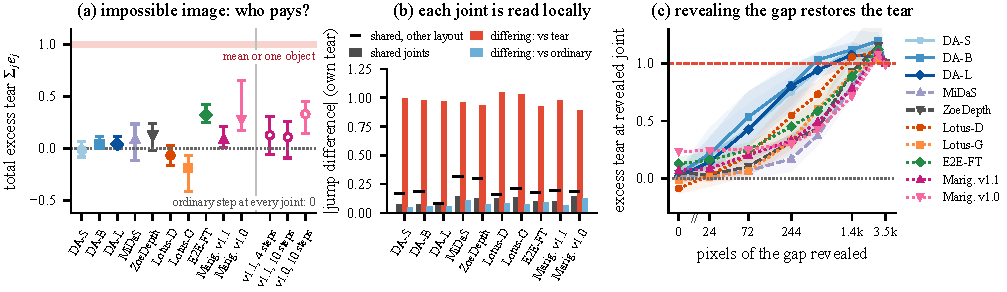
\includegraphics[width=\textwidth]{fig_main.pdf}
\caption{\textbf{No joint pays for the impossibility.} (a) Total excess tear on the impossible image (median, 95\%
cluster-bootstrap interval over layouts; samplers: all seeds; hollow: Marigold with 4 or 10 DDIM steps);
the mean or one object gives 1. (b) Jump
difference between the impossible image and its matched control, in units of the network's tear, at the two shared joints (tick: a control
$45^\circ$ away) and at the differing joint, compared with the control's jump and with that joint's ordinary step. (c) Excess
tear at the revealed joint vs pixels revealed (bands: 90\% intervals; at $\tau=1$, the control, $e=1$ by definition). DA = Depth Anything V2; Marig.\ = Marigold; terms as in Sec.~\ref{sec:readout}.}
\label{fig:main}
\end{figure*}

\subsection{What an ideal predictor returns}\label{sec:theory}
Let the predictor's belief put weight $p_k$ on object $k$. Read around the loop in the order of Fig.~\ref{fig:hero}, $d_k$ comes nearer at a constant rate along the bars and jumps back by $T$ at joint $k$.
\begin{proposition}
For a squared error with targets that do not depend on the prediction (Lotus and Marigold normalise each target on its
own), the optimum is $\sum_kp_kd_k$, which jumps by $p_kT$ at joint $k$.
\end{proposition}
\begin{proposition}
For a per-pixel absolute error the optimum is $d_k$ if $p_k>1/2$. If every $p_k<1/2$ and each object is median-centred, the optimum is the middle of the three values, which on every bar is their mean: it jumps by $T/3$ at every
joint.
\end{proposition}
With least-squares scale-and-shift alignment an absolute error returns one object or the middle map, and so does Depth Anything's loss unless its gradient term is trimmed too (a squared error would return
the posterior's principal component, which can flatten the bars, but none of our networks uses it). The one-step output of a diffusion model is the posterior mean
given its starting noise~\cite{efron2011tweedie}, which is the mean given the image when the schedule reaches zero
signal~\cite{lin2024flawed}, as in Marigold v1.1 (derivations and numerical searches in the repository).
\begin{corollary}
The mean and each object share the objects' slope on every bar, so they pay the whole mismatch at the joints,
whatever $p$ is.
\end{corollary}
\noindent Near a two-way tie, the trimmed MiDaS loss prefers maps that stitch two objects, whose joints pay even more.

\subsection{Reading the loop}\label{sec:readout}
We take each cube's median depth over pixels at least 3\,px inside it, fit a line to each bar's four interior cubes,
and define the jump $J_j$ at joint $j$ as the next bar's line minus the previous bar's line, both extended to the joint;
the corner cubes, where junctions are drawn, are not used. A network's own possible controls at the same layout (or the nearest below; controls are $15^\circ$ apart) give, for every joint, its ordinary step $r_j$ (averaged over the two controls whose gap is elsewhere) and its step $g_j$ as the gap; $g_j-r_j$ is its tear. The excess tear
$e_j=(J_j-r_j)/(g_j-r_j)$ is invariant to a depth shift and to a scale shared by an image and its controls. The mean
has $e=p$ and one object has $e$ one-hot, so both have $\sum_je_j=1$; making the ordinary step at every joint gives
$e=0$. Ordinary steps are not zero: every network steps toward the viewer at ordinary joints, so a map with no jump
would total 0.21 (Depth Anything V2-L) to 1.29 (MiDaS). Comparing with 1 assumes that a network believing in object
$k$ returns what it returns on object $k$'s control. On the ground truth the read-out is accurate to 1\%; other erosions
(1 or 5\,px) or means instead of medians move $\sum_je_j$ by at most $0.11$ (seven networks re-read).

\subsection{Networks}
We run ten frozen public checkpoints: Depth Anything V2 S/B/L~\cite{yang2024dav2}, MiDaS DPT-L~\cite{ranftl2021dpt,
ranftl2022midas} and ZoeDepth~\cite{bhat2023zoedepth}, which use absolute or log errors, and five networks that share
the Stable Diffusion 2 (SD2) backbone~\cite{rombach2022ldm}, VAE and synthetic training data: Lotus-D and
Lotus-G~\cite{he2025lotus} (one step, squared error in the latent), Marigold E2E-FT~\cite{garcia2025finetuning} (one
step, least-squares-aligned absolute error) and Marigold v1.0/v1.1~\cite{ke2024marigold,ke2025marigold} (DDIM
samplers~\cite{song2021ddim}; one step unless stated). Lotus-G and Marigold v1.0/v1.1 ran with 32 noise seeds, one sample each, on all controls
and morph images but on 16 of the impossible images (8 layouts $\times$ 2 chiralities). A network is analysed if, on
the possible controls, its largest jump back sits at the gap in at least 80\% of images; all ten pass (nine above 99\%, MiDaS
88\%).

\section{Results}

\paragraph{On the impossible image the joints pay little.}
The total excess tear is far below 1 for every network (Fig.~\ref{fig:main}a): $-0.02$, $0.04$ and $0.04$ for Depth
Anything S/B/L, $0.09$ and $0.12$ for MiDaS and ZoeDepth, $-0.07$ for Lotus-D, $-0.19$ for Lotus-G and $0.09$ for
Marigold v1.1, against $0.32$ and $0.27$ for E2E-FT and Marigold v1.0, from which E2E-FT is fine-tuned. Per network, the median largest single-joint excess is 0.06--0.24. Since jumps and bar changes sum to zero around the loop, the mismatch the joints do not pay must go into
the bars; for Depth Anything and Lotus-D, whose mean bar slope follows the objects' on the controls, they reverse it.

\paragraph{What the totals rule out.}
Marigold v1.1's one-step output estimates its posterior mean; averaged over seeds it totals 0.10 (v1.0: 0.24), so it
is not the mean of any belief over the three objects. A belief that also admits their depth-reversed readings totals $P(\text{up})-P(\text{rev})$, which can be near 0. If a network reads a reversed object as its upright reading negated, such a mixture gives the ordinary step at every joint only if the three ordinary steps add up to at most half a tear. That holds for Depth Anything V2-B and V2-L, which would need a mostly reversed belief ($P(\text{rev})-P(\text{up})=0.57$, $0.27$) though both read the controls upright; V2-S and Lotus-D are at the bound. Per-bar slopes are too noisy, even on controls, to test this.

\paragraph{Each joint is read locally.}
The impossible image differs from the possible control of object $k$ only at joint $k$. At the two joints they share,
every network gives nearly the same jump on both images, within 7--15\% of its tear, against 16--32\% (\mbox{DA-L} 8\%) for a control $45^\circ$ away. At joint $k$ the tear disappears: the jump is 0.89--1.04 tears from the
control's but within 5--12\% of a tear of that joint's ordinary step (Fig.~\ref{fig:main}b).

\paragraph{Tens to hundreds of pixels restore the tear.}
Revealing the real gap brings the tear back smoothly (Fig.~\ref{fig:main}c). Depth Anything recovers half of its tear
from 64--95 changed pixels (under 0.04\% of the image); the SD2 networks need 207 (Lotus-D) to 669 (Marigold v1.0)
pixels, and MiDaS and ZoeDepth 688 and 588. Where the loop breaks is decided by what is visible at one junction.

\paragraph{Sampling does not commit either.}
A sampler that draws from a belief over the three objects returns one object per sample, each with $\sum_je_j=1$.
With 4 and 10 DDIM steps (64 seeds on 4 layouts; references: 16 seeds, same sampler), Marigold v1.1's samples total 0.13
and 0.11 (seed s.d. 0.2) and only 5--6\% pay half a tear or more; v1.0 at 10 steps totals 0.33 and 26\% do (Fig.~\ref{fig:main}a,
hollow). Along the trajectory v1.1's clean-image estimate stays at 0.01--0.11 from the first step, while v1.0's falls from
0.55 to 0.33, and the morph restores half of v1.1's tear at about 500 pixels, as at one step.

\section{Discussion}\label{sec:disc}
Whatever their loss, the networks pay a small fraction of the mismatch that the mean or one object would pay,
until the gap at one junction is revealed. The simplest account is that the depth step at a junction is set
by the junction's appearance, and nothing ties it to the depth the bars have gained around the loop; the loop's
inconsistency is then left in the bars, where no optimum we found of the networks' losses for a belief over the three
objects puts it. A belief that allows the gap anywhere along the loop, inside the bars too, would leave it there (its
mean is flat), as would one closed loop with bent bars, the reading a generic-viewpoint prior
would favour~\cite{freeman1994generic}. Arguments that a regressor averages the explanations of an ambiguous
input~\cite{zhang2016colorful} presuppose a belief that covers them; here it seems not to be confined to the three rigid
objects.

\paragraph{Limitations.}
The images are renders of one figure family, out of distribution for these networks, though every
network finds the gap of possible objects in the same style. Against the centred textured controls, the set-aside
images give totals of $-0.29$ to $0.60$, except MiDaS on untextured drawings (0.88). For the latent-diffusion networks Proposition 1 holds in latent space, so their predicted jumps are approximate.

\paragraph{Use of AI tools.} Claude assisted us with parts of the code and with drafting the text; we checked and approved all of it.

{\small
\bibliographystyle{plainnat}
\bibliography{refs}
}
\end{document}
